\chapter{Ejercicio 3: Histograma}

\section{Introducción}

    El cálculo del histograma es una operación fundamental en el procesamiento de imágenes y el análisis de datos, que proporciona una representación visual de la distribución de la frecuencia de los valores dentro de un conjunto de datos. En el contexto del procesamiento de imágenes, un histograma típicamente ilustra la distribución de la intensidad de los píxeles, donde el eje horizontal representa los posibles valores de intensidad (por ejemplo, de 0 a 255 en imágenes de escala de grises) y el eje vertical representa el número de píxeles en la imagen que poseen esa intensidad. Para conjuntos de datos generales, un histograma puede representar la frecuencia de cualquier tipo de valor.
    
    Esta representación es crucial para una variedad de aplicaciones. En el procesamiento de imágenes, los histogramas se utilizan para técnicas como la ecualización de histogramas, que mejora el contraste de una imagen distribuyendo más uniformemente las intensidades de los píxeles. También son esenciales en la segmentación de imágenes, donde el análisis de los picos y valles en un histograma puede ayudar a identificar regiones de interés o separar objetos del fondo. Además, los histogramas juegan un papel importante en el reconocimiento de objetos, ya que las características del histograma de una región de una imagen pueden servir como descriptores para identificar objetos o patrones. En el análisis estadístico de datos, los histogramas permiten visualizar la distribución de los datos, identificar valores atípicos y comprender la dispersión y la tendencia central de los datos.
    
    El cálculo del histograma se caracteriza por su naturaleza inherentemente paralela, ya que el procesamiento de cada elemento de los datos (ya sea un píxel en una imagen o un punto de datos en un conjunto de datos) puede contribuir independientemente al conteo de su correspondiente ``bin'' o intervalo en el histograma. Esta independencia permite que el cálculo del histograma se beneficie enormemente de las arquitecturas de computación paralela, como las GPUs. Sin embargo, el cálculo del histograma también presenta desafíos significativos, especialmente en implementaciones paralelas. Uno de los principales desafíos es la gestión eficiente de la memoria, ya que el histograma en sí debe almacenarse y actualizarse de manera eficiente. Además, cuando múltiples hilos de ejecución intentan actualizar simultáneamente el conteo de un mismo \textit{bin}, pueden ocurrir condiciones de carrera, lo que requiere el uso de mecanismos de sincronización para garantizar la corrección de los resultados.
    
    Este apartado presenta dos implementaciones del algoritmo del histograma utilizando CUDA, una plataforma de computación paralela de NVIDIA: una implementación que utiliza memoria global y otra que utiliza memoria compartida. La memoria global es la memoria principal de la GPU, accesible por todos los hilos, pero con una latencia relativamente alta. La memoria compartida, por otro lado, es una memoria \textit{on-chip}, mucho más rápida que la memoria global, pero de menor tamaño y accesible solo por los hilos dentro de un mismo bloque. Se analizará exhaustivamente el rendimiento de ambas implementaciones en la GPU NVIDIA A100, disponible en el centro de supercomputación CESGA. Se examinará no solo el rendimiento bruto de las implementaciones, sino también aspectos críticos como la escalabilidad (cómo se comporta el rendimiento al aumentar el tamaño de los datos), la eficiencia de utilización de los recursos de la GPU (como los multiprocesadores y la memoria), y las compensaciones entre diferentes estrategias de gestión de memoria (memoria global vs. memoria compartida) para identificar las estrategias óptimas de implementación del cálculo del histograma en arquitecturas paralelas.

\newpage

\section{Fundamentos teóricos}

    \subsection{Algoritmo de cálculo de histogramas}

        El cálculo de histogramas es una operación fundamental en el procesamiento de imágenes y análisis de datos. Dado un conjunto de valores (en este caso, los píxeles de una imagen en escala de grises), el histograma cuenta la frecuencia de cada valor en un rango predefinido (por ejemplo, 0 a 255 para imágenes de 8 bits). Matemáticamente, el histograma se define como:

        \begin{align}
            H[i] = \sum_{j=0}^{N-1} \delta(I[j], i), \quad \text{para } i = 0, 1, \ldots, L-1
        \end{align}

        Donde:

        \begin{itemize}
        
            \item \( I \) es el vector de píxeles de la imagen.
            
            \item \( N \) es el número total de píxeles en la imagen.
            
            \item \( L \) es el número de niveles de gris (por ejemplo, 256 para imágenes de 8 bits).
            
            \item \( \delta(I[j], i) \) es una función delta que devuelve 1 si \( I[j] = i \) y 0 en caso contrario.
            
        \end{itemize}

        El cálculo del histograma es una operación que se puede paralelizar eficientemente en GPU, ya que cada píxel puede ser procesado de manera independiente. Sin embargo, la acumulación de los valores en el histograma requiere sincronización para evitar condiciones de carrera. Esto se debe a que múltiples hilos pueden intentar actualizar el mismo contador del histograma simultáneamente, lo que podría llevar a resultados incorrectos si no se maneja adecuadamente.

        \subsubsection{Propiedades del cálculo de histogramas}

            El cálculo de histogramas presenta las siguientes propiedades computacionales:
            
            \begin{itemize}
            
                \item \textbf{Independencia de datos}: Cada píxel puede ser procesado de manera independiente, lo que permite una paralelización perfecta. Sin embargo, la acumulación de los conteos en el histograma global requiere sincronización.
                
                \item \textbf{Intensidad aritmética baja}: El cálculo de histogramas es una operación \textit{memory-bound}, ya que implica más accesos a memoria que operaciones aritméticas. Cada píxel requiere una lectura de memoria y una actualización del contador correspondiente en el histograma.
               
                \item \textbf{Patrones de acceso irregulares}: A diferencia de algoritmos como DAXPY, donde los accesos a memoria son secuenciales, el cálculo de histogramas implica accesos aleatorios a los contadores del histograma, lo que puede generar contención en la memoria global.
                
            \end{itemize}

    \subsection{Memoria global en CUDA}

        La memoria global en CUDA es la memoria principal de la GPU, accesible por todos los hilos de todos los bloques. Es la memoria más grande disponible en la GPU, pero también es la más lenta en términos de latencia y ancho de banda en comparación con otros tipos de memoria como la memoria compartida o los registros. En el contexto del cálculo de histogramas, la memoria global se utiliza para almacenar la imagen de entrada y el histograma final.

        \subsubsection{Características de la memoria global}

            \begin{itemize}
               
                \item \textbf{Alto ancho de banda, alta latencia}: Aunque la memoria global tiene un ancho de banda considerable, su latencia es alta. Para mitigar esto, es crucial optimizar los patrones de acceso a memoria.
                
                \item \textbf{Acceso coalescente}: Para maximizar el rendimiento, los accesos a la memoria global deben ser coalescentes, es decir, los hilos dentro de un mismo \textit{warp} deben acceder a posiciones de memoria contiguas. Esto permite que el \textit{hardware} consolide múltiples accesos en una sola transacción de memoria.
               
                \item \textbf{Uso de operaciones atómicas}: En el cálculo de histogramas, la memoria global se utiliza para almacenar el histograma final. Dado que múltiples hilos pueden actualizar el mismo contador, es necesario utilizar operaciones atómicas para garantizar la coherencia. Sin embargo, el uso excesivo de operaciones atómicas puede generar contención y reducir el rendimiento.
                
            \end{itemize}
        
        \subsubsection{Optimización del acceso a la memoria global}
        
            Para optimizar el acceso a la memoria global en el cálculo de histogramas, se pueden aplicar las siguientes técnicas:
            
            \begin{itemize}
                
                \item \textbf{Coalescencia de accesos}: Asegurar que los hilos dentro de un mismo \textit{warp} accedan a posiciones de memoria contiguas. Esto se logra organizando los datos de manera que los hilos procesen elementos consecutivos del vector de entrada.
                
                \item \textbf{\textit{Prefetching}}: Anticipar los accesos a memoria para reducir la latencia. Esto se puede lograr utilizando técnicas como \texttt{cudaMemPrefetchAsync} para mover los datos a la GPU antes de que sean necesarios.
                
                \item \textbf{Reducción de la contención atómica}: Minimizar el uso de operaciones atómicas en la memoria global utilizando técnicas como la reducción paralela en memoria compartida antes de actualizar el histograma global.
          
            \end{itemize}

    \subsection{Memoria compartida en CUDA}

        La memoria compartida es un recurso crítico en CUDA para optimizar el rendimiento de algoritmos como el cálculo de histogramas. Es una memoria de alta velocidad que es accesible por todos los hilos dentro de un mismo bloque. Su uso permite reducir los accesos a la memoria global, que es más lenta, y mejorar el rendimiento general del \textit{kernel}.

        \subsubsection{Características de la memoria compartida}
        
            \begin{itemize}
                
                \item \textbf{Baja latencia}: La memoria compartida es mucho más rápida que la memoria global, con tiempos de acceso similares a los de los registros.
                
                \item \textbf{Acceso por bloque}: Cada bloque de hilos tiene su propia región de memoria compartida, que no es accesible por hilos de otros bloques.
                
                \item \textbf{Limitada en tamaño}: La memoria compartida es un recurso limitado. En la mayoría de las GPU modernas, cada bloque puede utilizar hasta 48 KB de memoria compartida. Esto significa que su uso debe ser cuidadosamente planificado para evitar agotar este recurso.
          
            \end{itemize}
        
        \subsubsection{Uso de la memoria compartida}
        
            En el cálculo de histogramas, la memoria compartida se utiliza para acumular los conteos parciales de cada bloque antes de combinarlos en el histograma global. Esto reduce la contención en la memoria global y mejora el rendimiento. La estrategia típica es:
            
            \begin{enumerate}
            
                \item Cada bloque de hilos calcula un histograma parcial en memoria compartida.
                
                \item Los histogramas parciales se combinan en el histograma global utilizando operaciones atómicas para garantizar la coherencia.
                
            \end{enumerate}
        
        \subsubsection{Optimización usando memoria compartida}
        
            Para optimizar el uso de la memoria compartida en el cálculo de histogramas, se pueden aplicar las siguientes técnicas:
            
            \begin{itemize}
            
                \item \textbf{Reducción de la contención}: Dividir el histograma en múltiples bancos para reducir la contención en los accesos a memoria compartida. Esto es especialmente útil cuando múltiples hilos intentan actualizar el mismo contador.
                
                \item \textbf{Uso eficiente del espacio}: Asegurar que la memoria compartida se utilice de manera eficiente, evitando el desperdicio de espacio. Por ejemplo, en el cálculo de histogramas, se puede utilizar un \textit{array} de tamaño fijo (256 elementos para imágenes de 8 bits) para almacenar los conteos parciales.
              
                \item \textbf{Sincronización entre hilos}: Utilizar \texttt{\_\_syncthreads()} para garantizar que todos los hilos dentro de un bloque hayan terminado de actualizar el histograma parcial antes de combinarlo en el histograma global.
            
            \end{itemize}

    \subsection{Configuración de bloques e hilos}
    
        La organización de los hilos en bloques y \textit{grids} es crucial para el rendimiento del cálculo de histogramas en CUDA. La configuración óptima depende del tamaño de la imagen y de las características del \textit{hardware}. En general, se busca maximizar la ocupación de los multiprocesadores (SMs) de la GPU, lo que se logra equilibrando el número de hilos por bloque y el número de bloques por \textit{grid}.
        
        \begin{lstlisting}[language=C, caption={Calculo de dimensiones de bloques y \textit{grid}.}, gobble=12]
            int threadsPerBlock = atoi(argv[2]);
            long blocksPerGrid = ceil(imageSize / threadsPerBlock);
        \end{lstlisting}
                
        Donde:
        
        \begin{itemize}
        
            \item \texttt{threadsPerBlock} es el número de hilos por bloque.
            
            \item \texttt{blocksPerGrid} es el número de bloques necesarios para cubrir todos los píxeles de la imagen.
            
        \end{itemize}

        \subsubsection{Consideraciones arquitectónicas}
        
            \begin{itemize}
            
                \item \textbf{Granularidad de los bloques}: El número de hilos por bloque determina la unidad básica de trabajo que se asigna a cada SM. Bloques más grandes pueden maximizar la utilización de recursos, pero podrían limitar el número de bloques concurrentes por SM.
                
                \item \textbf{Eficiencia de \textit{warps}}: Dado que los \textit{warps} son unidades de 32 hilos, tamaños de bloque que no sean múltiplos exactos de 32 resultarán en \textit{warps} parcialmente ocupados, desperdiciando capacidad computacional.
                
                \item \textbf{Balanceo de carga}: Un número suficientemente grande de bloques asegura que todos los SMs disponibles reciban trabajo, maximizando la utilización global de la GPU.
                
            \end{itemize}
        
    \subsection{Patrones de acceso a memoria}

        El rendimiento del cálculo de histogramas en GPU está fuertemente influenciado por los patrones de acceso a memoria. Para maximizar la eficiencia, es importante garantizar que los accesos a memoria global sean coalescentes, es decir, que los hilos dentro de un mismo \textit{warp} accedan a posiciones de memoria contiguas. Esto permite que el \textit{hardware} consolide múltiples accesos en una sola transacción de memoria.
        
        \subsubsection{Coalescencia de accesos}

            La coalescencia de accesos es fundamental para maximizar el rendimiento en arquitecturas GPU. Cuando los hilos dentro de un mismo \textit{warp} acceden a posiciones de memoria contiguas, el \textit{hardware} puede consolidar estos accesos en un número mínimo de transacciones de memoria, aprovechando al máximo el ancho de banda disponible.

        \subsubsection{Distribución cíclica mediante \textit{stride}}

            La utilización de un \textit{stride} igual al número total de hilos distribuye el trabajo cíclicamente entre todos los hilos disponibles. Esta estrategia presenta ventajas arquitectónicas significativas, como el balanceo de carga intrínseco y la amortización del \textit{overhead} de lanzamiento.

    \subsection{Análisis de ocupancia y rendimiento}

        La ocupancia es una métrica clave en CUDA que mide la proporción de recursos computacionales que están siendo utilizados activamente en comparación con el máximo teórico. Para el cálculo de histogramas, una alta ocupancia no siempre se traduce en un mejor rendimiento, ya que el algoritmo está limitado por el ancho de banda de memoria.
        
        \subsubsection{Cálculo de la ocupancia}

            La ocupancia se calcula utilizando la API de CUDA:
            
            \begin{lstlisting}[language=C, caption={Calculo de ocupancia teorica.}, gobble=16]
                int maxBlocksPerSM;
                cudaOccupancyMaxActiveBlocksPerMultiprocessor(&maxBlocksPerSM, histogram, threadsPerBlock, 0);
                float occupancy = (float)(maxBlocksPerSM * threadsPerBlock) / prop.maxThreadsPerMultiProcessor;
            \end{lstlisting}
            
            Donde:
            
            \begin{itemize}
            
                \item \texttt{maxBlocksPerSM} es el número máximo de bloques que pueden alocarse y ejecutarse simultáneamente en un multiprocesador de NVIDIA.

                \item \texttt{threadsPerBlock} es el número de hilos por bloque.

                \item \texttt{prop.maxThreadsPerMultiProcessor} es el número máximo de hilos que un multiprocesador puede manejar.
                
            \end{itemize}

    \subsection{Limitaciones y optimizaciones}

        A pesar de las optimizaciones, el cálculo de histogramas en GPU tiene limitaciones inherentes debido a la naturaleza del algoritmo. Algunas de estas limitaciones incluyen:
        
        \begin{itemize}
        
            \item \textbf{Contención en operaciones atómicas}: La acumulación de los conteos en el histograma global requiere el uso de operaciones atómicas, lo que puede generar contención y reducir el rendimiento.
            
            \item \textbf{Uso de memoria compartida}: La memoria compartida es un recurso limitado, y su uso excesivo puede reducir el número de bloques que se pueden ejecutar simultáneamente.
            
            \item \textbf{Ancho de banda de memoria}: El algoritmo está limitado por el ancho de banda de memoria, especialmente en imágenes grandes.
            
        \end{itemize}

        \subsubsection{Optimizaciones potenciales}
    
            Algunas optimizaciones potenciales incluyen:
            
            \begin{itemize}
            
                \item \textbf{Reducción de la contención atómica}: Utilizar técnicas como la reducción paralela para combinar los histogramas parciales antes de realizar operaciones atómicas en el histograma global.
                
                \item \textbf{Uso eficiente de la memoria compartida}: Optimizar el uso de la memoria compartida para maximizar la ocupación y reducir la contención.
                
                \item \textbf{\textit{Prefetching} de datos}: Anticipar los accesos a memoria para reducir la latencia.
                
            \end{itemize}
    
            Estas optimizaciones pueden mejorar significativamente el rendimiento del cálculo de histogramas en GPU, especialmente en aplicaciones de procesamiento de imágenes a gran escala.

\newpage

\section{Implementación}

    El cálculo de histogramas es una operación fundamental en el procesamiento de imágenes y análisis de datos, que consiste en contar la frecuencia de ocurrencia de cada valor en un conjunto de datos. En este caso, se ha implementado en CUDA utilizando dos enfoques distintos: uno que utiliza memoria global y otro que aprovecha la memoria compartida para optimizar el rendimiento. A continuación, se presenta un análisis detallado de ambas implementaciones, examinando las decisiones de diseño, las implicaciones arquitectónicas y las diferencias clave entre los dos enfoques.

    \subsection{Estructura general}
    
        Ambas implementaciones siguen una estructura modular que facilita la comprensión, el mantenimiento y la optimización del código. Los componentes principales incluyen:
        
        \begin{enumerate}
        
            \item \textbf{Funciones de utilidad}: Incluyen mecanismos para la medición precisa de tiempos utilizando \texttt{CLOCK\_MONOTONIC}, que proporciona una resolución de nanosegundos y es inmune a ajustes del sistema. Además, se incluyen rutinas de comprobación de errores que verifican las llamadas a la API de CUDA, garantizando la integridad de la ejecución y facilitando la depuración.
            
            \item \textbf{\textit{Kernel} de histograma}: El núcleo computacional del programa, implementa el cálculo del histograma de forma paralela. En una versión se utiliza memoria global, mientras que en la otra se aprovecha la memoria compartida para optimizar el rendimiento.
            
            \item \textbf{Implementación secuencial en CPU}: Una versión optimizada para CPU que sirve tanto para la verificación de resultados como para establecer una referencia de rendimiento. Esta implementación es esencial para garantizar la corrección de los resultados obtenidos en la GPU.
            
            \item \textbf{Función principal}: Coordina la ejecución de los diferentes componentes, gestiona la configuración de los parámetros de ejecución (como el número de \textit{threads} por bloque) y realiza mediciones detalladas de rendimiento. Además, se encarga de la asignación y liberación de memoria tanto en la CPU como en la GPU.
            
        \end{enumerate}

        Esta estructura no solo facilita la comprensión del código, sino que también permite aislar y medir con precisión el rendimiento de cada componente del sistema, identificando posibles cuellos de botella y oportunidades de optimización.

    \subsection{Gestión de memoria}

        La gestión de memoria es un aspecto crítico en el rendimiento de aplicaciones CUDA, especialmente en operaciones como el cálculo de histogramas, donde se realizan numerosos accesos a memoria. Ambas implementaciones utilizan la API de CUDA para asignar y transferir datos entre la CPU y la GPU, pero difieren en cómo manejan la memoria dentro del \textit{kernel}.
        
        \subsubsection{Memoria global en \texttt{histogram\_1.cu}}

            En la primera implementación (\texttt{histogram\_1.cu}), el \textit{kernel} utiliza memoria global para almacenar el histograma local de cada \textit{thread}. Esto implica que cada \textit{thread} accede directamente a la memoria global para actualizar el histograma, lo que puede resultar en un alto número de accesos a memoria y posibles contenciones en las operaciones atómicas.
            
            \begin{itemize}
            
                \item \textbf{Histograma local por \textit{thread}}: Cada \textit{thread} mantiene su propio histograma local en un \textit{array} en memoria global. Esto permite que los \textit{threads} trabajen de forma independiente, pero también implica que cada \textit{thread} debe realizar múltiples accesos a la memoria global, lo que puede ser costoso en términos de rendimiento.
                
                \item \textbf{Acceso coalescente}: Los \textit{threads} acceden a posiciones de memoria contiguas en el \textit{array} de entrada, lo que maximiza la eficiencia de las transacciones de memoria. Sin embargo, los accesos al histograma global no son coalescentes, ya que los \textit{threads} pueden actualizar \textit{bins} diferentes de forma aleatoria.
                
                \item \textbf{Actualización atómica}: Los \textit{threads} utilizan operaciones atómicas para actualizar el histograma global, lo que garantiza la corrección en presencia de múltiples \textit{threads} que actualizan el mismo \textit{bin}. Sin embargo, las operaciones atómicas pueden generar contención y reducir el rendimiento, especialmente cuando muchos \textit{threads} intentan actualizar el mismo \textit{bin} simultáneamente.
                
            \end{itemize}
                    
        \subsubsection{Memoria compartida en \texttt{histogram\_2.cu}}
        
            En la segunda implementación (\texttt{histogram\_2.cu}), el \textit{kernel} utiliza memoria compartida para almacenar un histograma local por bloque. Esto reduce el número de accesos a la memoria global y mejora la eficiencia al permitir que los \textit{threads} dentro de un bloque colaboren en la construcción del histograma antes de realizar una única actualización atómica en la memoria global.
        
            \begin{itemize}
            
                \item \textbf{Histograma local por bloque}: Cada bloque mantiene un histograma local en memoria compartida, lo que reduce el número de accesos a la memoria global. La memoria compartida es mucho más rápida que la memoria global, lo que permite a los \textit{threads} actualizar el histograma local de forma eficiente.
                
                \item \textbf{Inicialización de memoria compartida}: Los \textit{threads} dentro de un bloque inicializan el histograma compartido en paralelo, lo que mejora la eficiencia. Cada \textit{thread} es responsable de inicializar una porción del histograma compartido, lo que permite una distribución uniforme del trabajo.
                
                \item \textbf{Actualización atómica en memoria compartida}: Los \textit{threads} utilizan operaciones atómicas para actualizar el histograma compartido, lo que garantiza la corrección en presencia de múltiples \textit{threads} dentro del mismo bloque. Aunque las operaciones atómicas en memoria compartida también pueden generar contención, esta contención es limitada a los \textit{threads} dentro del mismo bloque, lo que reduce su impacto en el rendimiento global.
                
                \item \textbf{Actualización atómica en memoria global}: Una vez que el histograma compartido está completo, los \textit{threads} actualizan el histograma global utilizando operaciones atómicas. Esta actualización se realiza de forma más eficiente, ya que cada bloque realiza una única actualización atómica por \textit{bin} en lugar de múltiples actualizaciones atómicas por \textit{thread}.
                
            \end{itemize}
            
    \subsection{\textit{Kernel} con memoria global}
        
        El \textit{kernel} en \texttt{histogram\_1.cu} utiliza memoria global para almacenar el histograma local de cada \textit{thread}. A continuación, se presenta un análisis detallado de su implementación:
        
        \begin{lstlisting}[language=C, caption={\textit{Kernel} usando memoria global.}, gobble=12]
            __global__ void histogram(unsigned char* input, int* histogram, size_t imageSize) {
                unsigned int localHistogram[GRAY_LEVELS] = {0};
            
                int tid = blockIdx.x * blockDim.x + threadIdx.x;
                int stride = blockDim.x * gridDim.x;
            
                for (int i = tid; i < imageSize; i += stride) {
                    localHistogram[input[i]]++;
                }
            
                for (int binIdx = 0; binIdx < GRAY_LEVELS; binIdx++) {
                    if (localHistogram[binIdx] > 0) {
                        atomicAdd(&histogram[binIdx], localHistogram[binIdx]);
                    }
                }
            }
        \end{lstlisting}

        \subsubsection{Análisis del \textit{kernel}}

            \begin{itemize}
            
                \item \textbf{Paralelismo}: Cada \textit{thread} procesa una porción del \textit{array} de entrada, lo que permite una distribución uniforme del trabajo. El uso de un bucle con \texttt{stride} garantiza que todos los \textit{threads} contribuyan al cálculo del histograma, incluso cuando el número de \textit{threads} es menor que el tamaño del \textit{array} de entrada.
                
                \item \textbf{Histograma local}: Cada \textit{thread} mantiene su propio histograma local en un \textit{array} en memoria global. Esto permite que los \textit{threads} trabajen de forma independiente, pero también implica que cada \textit{thread} debe realizar múltiples accesos a la memoria global, lo que puede ser costoso en términos de rendimiento.
                
                \item \textbf{Actualización atómica}: Los \textit{threads} utilizan operaciones atómicas para actualizar el histograma global, lo que garantiza la corrección en presencia de múltiples \textit{threads} que actualizan el mismo \textit{bin}. Sin embargo, las operaciones atómicas pueden generar contención y reducir el rendimiento, especialmente cuando muchos \textit{threads} intentan actualizar el mismo \textit{bin} simultáneamente.
                
            \end{itemize}

    \subsection{\textit{Kernel} con memoria compartida}

        El \textit{kernel} en \texttt{histogram\_2.cu} utiliza memoria compartida para almacenar un histograma local por bloque. A continuación, se presenta un análisis detallado de su implementación:
        
        \begin{lstlisting}[language=C, caption={\textit{Kernel} usando memoria compartida.}, gobble=12]
            __global__ void histogram(unsigned char* input, int* globalHistogram, size_t imageSize) {
                __shared__ unsigned int sharedHistogram[GRAY_LEVELS];
            
                int tid = blockIdx.x * blockDim.x + threadIdx.x;
                int stride = blockDim.x * gridDim.x;
                int localThreadID = threadIdx.x;
            
                for (int i = localThreadID; i < GRAY_LEVELS; i += blockDim.x) {
                    sharedHistogram[i] = 0;
                }
            
                __syncthreads();
            
                for (int i = tid; i < imageSize; i += stride) {
                    unsigned char pixelValue = input[i];
                    atomicAdd(&sharedHistogram[pixelValue], 1);
                }
            
                __syncthreads();
            
                for (int i = localThreadID; i < GRAY_LEVELS; i += blockDim.x) {
                    if (sharedHistogram[i] > 0) {
                        atomicAdd(&globalHistogram[i], sharedHistogram[i]);
                    }
                }
            }
        \end{lstlisting}
        
        \subsubsection{Análisis del \textit{kernel}}
                        
            \begin{itemize}

                \item \textbf{Inicialización del histograma compartido}:  Cada \textit{thread} dentro de un bloque es responsable de inicializar una porción del histograma compartido. Esto se realiza en paralelo, lo que permite una distribución uniforme del trabajo. La inicialización se divide entre los \textit{threads} del bloque, donde cada \textit{thread} inicializa un subconjunto de los \textit{bins} del histograma. Esto es más eficiente que asignar la inicialización a un solo \textit{thread}, ya que se aprovecha el paralelismo dentro del bloque.
                
                \item \textbf{Uso de \texttt{\_\_syncthreads()}}: Después de la inicialización del histograma compartido, se llama a `\_\_syncthreads()`. Esta función es una barrera de sincronización que garantiza que todos los \textit{threads} dentro del bloque hayan completado la inicialización antes de que cualquier \textit{thread} proceda a la siguiente fase del cálculo. Esto es crucial para evitar condiciones de carrera, donde un \textit{thread} podría intentar leer o escribir en el histograma compartido antes de que otro \textit{thread} haya terminado de inicializarlo.
                
                \item \textbf{Cálculo del histograma local en memoria compartida}: Una vez que el histograma compartido está inicializado, los \textit{threads} comienzan a procesar el \textit{array} de entrada. Cada \textit{thread} procesa una porción del \textit{array} de entrada y actualiza el histograma compartido utilizando operaciones atómicas (\texttt{atomicAdd}). Estas operaciones atómicas garantizan que las actualizaciones al histograma compartido sean correctas incluso cuando múltiples \textit{threads} intentan actualizar el mismo \textit{bin} simultáneamente. Sin embargo, dado que la memoria compartida es mucho más rápida que la memoria global, la contención en las operaciones atómicas es menos costosa en términos de rendimiento.
                
                \item \textbf{Sincronización antes de la actualización global}: Después de que todos los \textit{threads} hayan terminado de procesar el \textit{array} de entrada y actualizar el histograma compartido, se llama nuevamente a \texttt{\_\_syncthreads()}. Esta segunda sincronización garantiza que todos los \textit{threads} dentro del bloque hayan completado sus contribuciones al histograma compartido antes de que cualquier \textit{thread} proceda a actualizar el histograma global. Esto es esencial para evitar que un \textit{thread} comience a actualizar el histograma global mientras otros \textit{threads} aún están procesando el \textit{array} de entrada.
                
                \item \textbf{Actualización del histograma global}: Finalmente, los \textit{threads} actualizan el histograma global utilizando operaciones atómicas. Cada \textit{thread} es responsable de actualizar una porción del histograma global, lo que permite una distribución uniforme del trabajo. La actualización se realiza de forma más eficiente que en la implementación que utiliza memoria global, ya que cada bloque realiza una única actualización atómica por \textit{bin} en lugar de múltiples actualizaciones atómicas por \textit{thread}.
                
            \end{itemize}
            
    \subsection{Configuración de ejecución}
    
        La configuración de ejecución en ambas implementaciones se determina dinámicamente según los parámetros de entrada:
        
        \begin{lstlisting}[language=C, caption={Calculo de las dimensiones del \textit{grid}.}, gobble=12]
            long blocksPerGrid = ceil(imageSize / threadsPerBlock);
        \end{lstlisting}
        
        Esta configuración permite explorar diferentes configuraciones de ejecución sin modificar el código fuente, facilitando la búsqueda de parámetros óptimos para cada combinación específica de hardware y tamaño de problema.
        
    \subsection{Medición de tiempos}
    
        Ambas implementaciones utilizan una función de alta precisión basada en el uso de \texttt{clock\_gettime} para medir el tiempo de cada fase crítica de la ejecución:
        
        \begin{lstlisting}[language=C, caption={Función de medición de tiempo.}, gobble=12]
            double get_time() {
                struct timespec ts;
                clock_gettime(CLOCK_MONOTONIC, &ts);
                return ts.tv_sec + ts.tv_nsec / 1.0e9;
            }
        \end{lstlisting}
    
        El programa mide meticulosamente el tiempo de cada fase crítica de la ejecución, incluyendo la asignación de memoria, la inicialización, la ejecución del \textit{kernel} y la transferencia de datos.
        
    \subsection{Verificación de resultados}
        
        Ambas implementaciones incluyen un mecanismo exhaustivo de verificación que compara los resultados obtenidos en la GPU con una implementación de referencia en CPU:
        
        \begin{lstlisting}[language=C, caption={Comprobación de errores.}, gobble=12]
            int errors = 0;
            for (int i = 0; i < GRAY_LEVELS; i++) {
                if (h_hist[i] != h_hist_cpu[i]) {
                    errors = 1;
                    break;
                }
            }
        \end{lstlisting}
        
        Este proceso de verificación garantiza la corrección de los resultados y proporciona información valiosa sobre la precisión de la implementación en GPU.

\newpage

\section{Resultados y análisis}
    
    \subsection{Introducción}

        En este apartado se analizan los resultados obtenidos en la implementación de algoritmos de histograma en GPU utilizando CUDA. Este análisis se centra en comparar dos implementaciones diferentes para el cálculo de histogramas: una basada en memoria global y otra que utiliza memoria compartida. Los histogramas son estructuras de datos fundamentales en el procesamiento de imágenes, que contabilizan la frecuencia de cada nivel de gris en una imagen.
        La implementación se ha realizado mediante dos \textit{kernels} CUDA distintos que procesan imágenes en formato PGM. El primer \textit{kernel} (\texttt{histogram\_1.cu}) utiliza exclusivamente memoria global con optimizaciones básicas como el uso de histogramas locales por \textit{thread} para reducir colisiones en los accesos atómicos. El segundo \textit{kernel} (\texttt{histogram\_2.cu}) implementa una versión más sofisticada que aprovecha la memoria compartida disponible en cada bloque de \textit{threads}, lo que potencialmente reduce la latencia de acceso a memoria y mejora el paralelismo.

        Para cada implementación, se ha medido el tiempo de ejecución dividido en diferentes fases: asignación de memoria (\texttt{alloc\_time}), inicialización (\texttt{init\_time}), cálculo del histograma (\texttt{histogram\_time}), transferencia de datos \textit{host-device} (\texttt{hd\_time}) y \textit{ device-host} (\texttt{dh\_time}). Adicionalmente, se calcula el tiempo total como la suma de todas estas fases. Las mediciones se han realizado variando el número de \textit{threads} por bloque (1, 2, 4, 8, 16, 32, 64, 128, 256, 512 y 1024) para estudiar su impacto en el rendimiento.

    \subsection{Escalabilidad}
    
        Las figuras \ref{fig:histogram_execution_times_global} y \ref{fig:histogram_execution_times_shared} presentan una evaluación cuantitativa del rendimiento de dos implementaciones algorítmicas divergentes para el cálculo de histogramas mediante CUDA: la primera basada en memoria global con reducción por thread y la segunda optimizada con memoria compartida utilizando reducción jerárquica por bloque. Ambas implementaciones fueron sometidas a evaluación utilizando un conjunto de imágenes de prueba con patrones estructurales específicos: gradientes por columnas, diagonal y filas, permitiendo analizar el impacto de la localidad espacial y los patrones de coherencia en acceso a datos.
        
        \begin{figure}[H]
            \centering
            \fbox{
                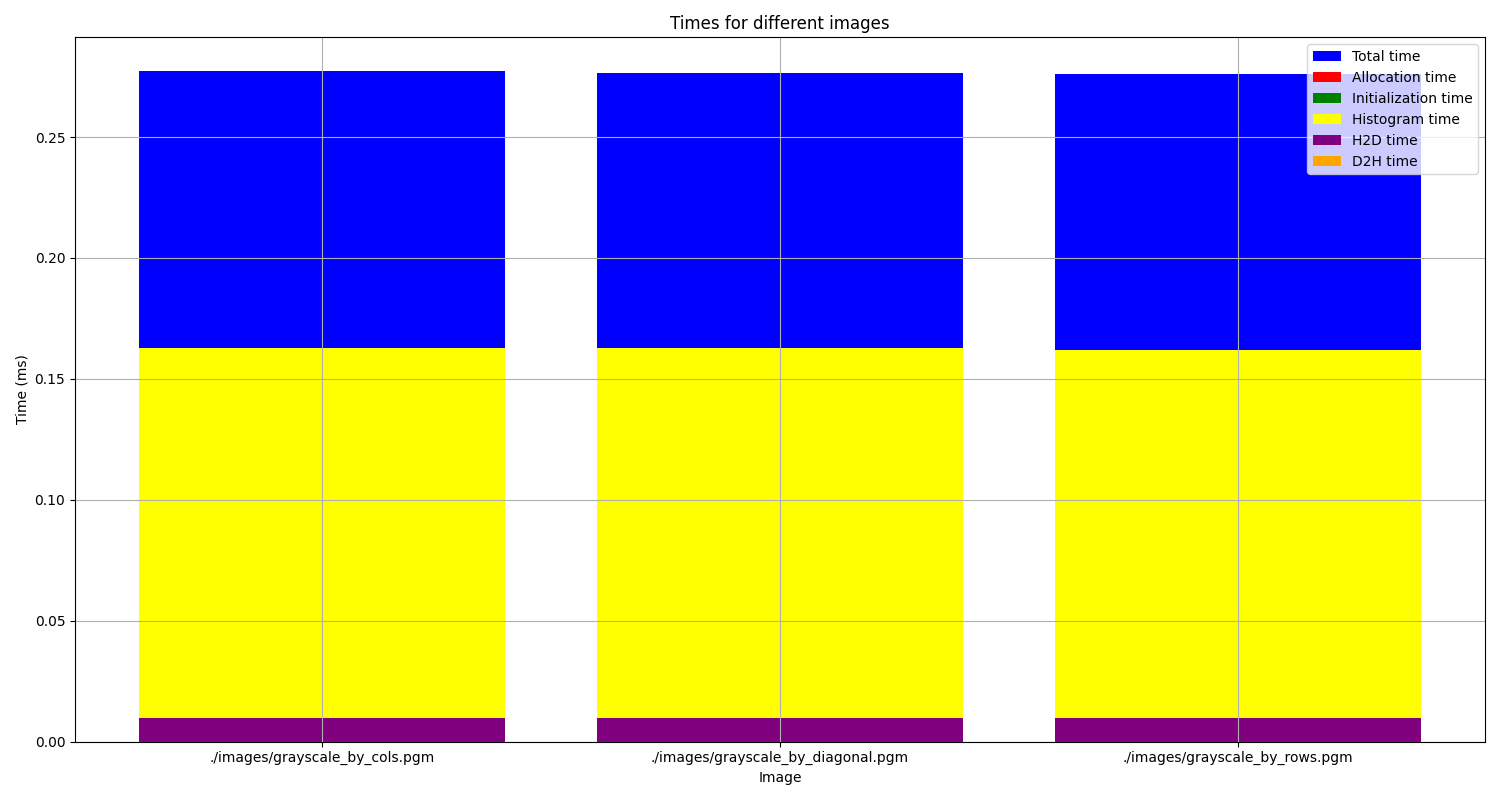
\includegraphics[width=0.9\textwidth]{images/histogram_1/execution_times.png}
            }
            \caption{Tiempos de ejecución según imagen usando memoria global.}
            \label{fig:histogram_execution_times_global}
        \end{figure}
        
        \begin{figure}[H]
            \centering
            \fbox{
                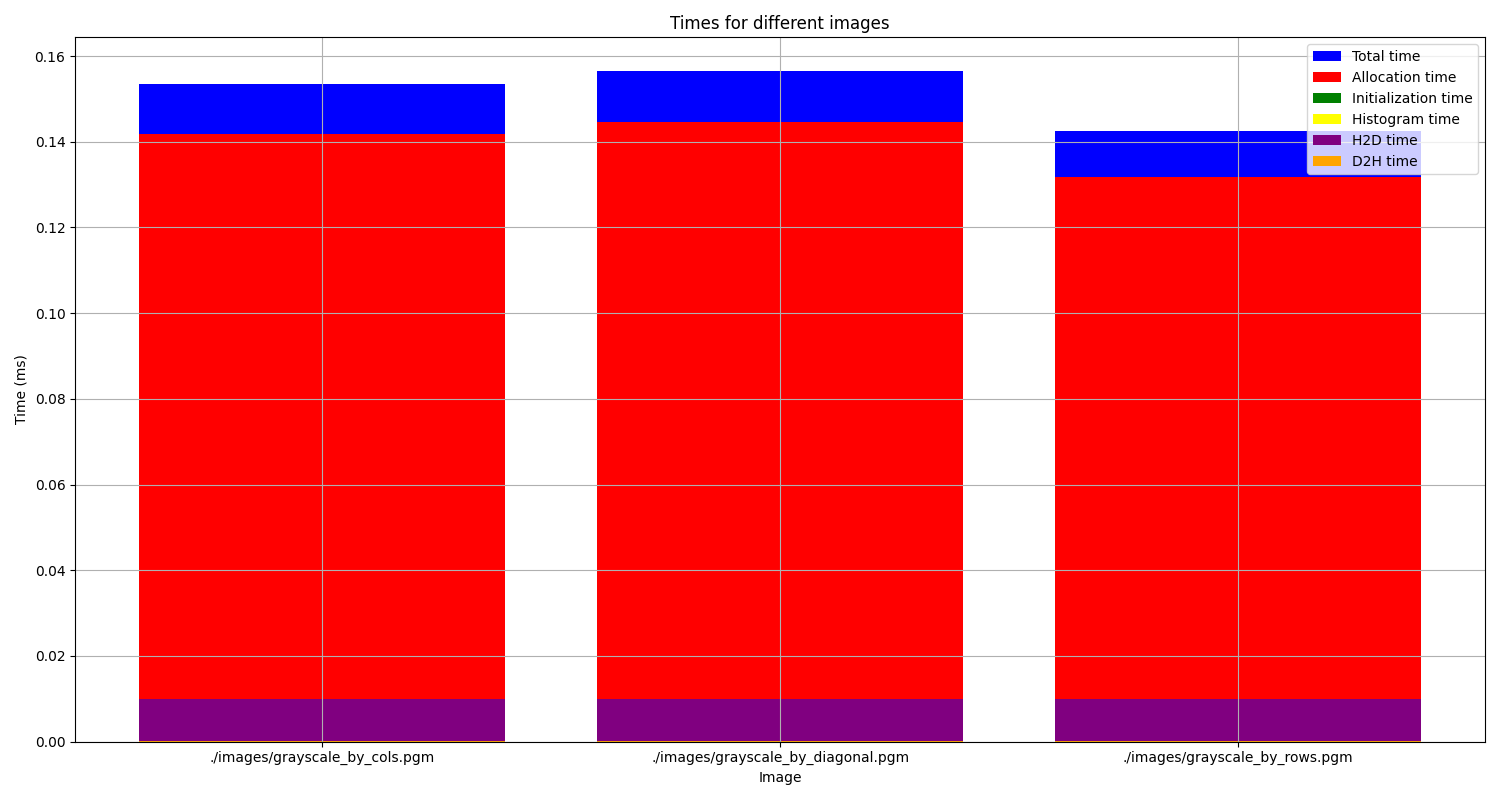
\includegraphics[width=0.9\textwidth]{images/histogram_2/execution_times.png}
            }
            \caption{Tiempos de ejecución según imagen usando memoria compartida.}
            \label{fig:histogram_execution_times_shared}
        \end{figure}

        En la implementación con memoria global (figura \ref{fig:histogram_execution_times_global}), se observa una distribución temporal donde el componente dominante es la ejecución del kernel de histograma (segmento amarillo), representando aproximadamente 0.17ms de los 0.27ms totales (63\%). Este comportamiento resulta de la arquitectura específica del \textit{kernel} \texttt{histogram} en \texttt{histogram\_1.cu}, que emplea el siguiente patrón de paralelismo:

        \begin{enumerate}

            \item \textbf{Reducción local con arrays registrados por \textit{thread}:} Cada \textit{thread} mantiene su propio histograma local completo (\texttt{unsigned int localHistogram[GRAY\_LEVELS] = {0}}) alojado en registros del SM (\textit{Streaming Multiprocessor}). 
            
            \item \textbf{Cómputo \textit{strided} con factor de \textit{stride} óptimo:} El patrón de acceso \texttt{for (int i = tid; i < imageSize; i += stride)} implementa un recorrido entrelazado que maximiza el rendimiento de la memoria global mediante transacciones coalescentes.
    
            \item \textbf{Fase de reducción con contención global:} La posterior consolidación haciendo uso de \texttt{atomicAdd(\&histogram[binIdx], localHistogram[binIdx])} introduce operaciones atómicas sobre memoria global que requieren serialización a nivel de SM.

        \end{enumerate}

        El análisis de rendimiento revela múltiples factores limitantes:

        \begin{enumerate}

            \item \textbf{Serialización multi-SM:} Las operaciones \texttt{atomicAdd} sobre memoria global inducen serialización entre threads de diferentes SM, provocando contención proporcional al número de threads concurrentes, escalando linealmente con la ocupancia CUDA.
        
            \item \textbf{Presión sobre el subsistema de memoria:} Cada \textit{bin} de histograma se convierte en un punto caliente de contención en la jerarquía de memoria, forzando invalidaciones de línea de caché L2 y generando tráfico de coherencia excesivo en el \textit{crossbar interconect}.

            \item \textbf{Divergencia SIMD (\textit{Single Instruction}, \textit{Multiple Data}):} La siguiente expresión condicional \texttt{if (localHistogram[binIdx] > 0)} introduce ejecución divergente en warps, degradando la eficiencia SIMT (\textit{Single Instruction}, \textit{Multiple Thread}) al subutilizar las unidades de ejecución vectorial.

            \item \textbf{Presión de registro:} El \textit{array} local \texttt{localHistogram[256]} requiere 1KB de espacio de registro por \textit{thread}, lo que puede reducir la ocupancia máxima teórica según el límite de registros por SM en la arquitectura específica.

        \end{enumerate}

        La escasa variación temporal entre las tres imágenes de prueba (< 2\%) indica que el rendimiento está dominado primordialmente por la contención en accesos atómicos, eclipsando cualquier efecto potencial derivado de los patrones espaciales de datos.
        
        La implementación con memoria compartida (figura \ref{fig:histogram_execution_times_shared}) exhibe una mejora de rendimiento sustancial, con una redistribución drástica del perfil temporal. El tiempo total se reduce a aproximadamente 0.15ms, representando una aceleración del 44.4\%. Notablemente, el segmento correspondiente al cálculo de histograma se reduce a una fracción casi imperceptible del tiempo total, mientras que la asignación de memoria (segmento rojo) domina ahora el perfil temporal.

        Esta optimización se fundamenta en sofisticadas técnicas de ingeniería de kernel en \texttt{histogram\_2.cu}:

        \begin{enumerate}

            \item \textbf{Particionamiento jerárquico de dominio:} La implementación realizada hace uso de 
 \texttt{\_\_shared\_\_ unsigned int sharedHistogram[GRAY\_LEVELS]} para crear histogramas parciales por bloque CUDA, reduciendo la contención atómica global al ámbito intra-bloque.
            
            \item \textbf{Inicialización vectorial cooperativa:} El siguiente patrón aplicado en el codigo \texttt{for (int i = localThreadID; i < GRAY\_LEVELS; i += blockDim.x)} implementa una inicialización entrelazada que aprovecha el ancho de banda de memoria compartida, cercano a los 9TB/s teóricos en arquitecturas recientes.
            
            \item \textbf{Paralelismo por fases con sincronización explícita:} Las directivas proporcionadas por NVIDIA \texttt{\_\_syncthreads()} crean puntos de sincronización que garantizan coherencia de memoria sin requerir instrucciones de barrera a nivel de \textit{warp} (\texttt{\_\_syncwarp()}).
            
            \item \textbf{Consolidación condicional selectiva:} La evaluación \texttt{if (sharedHistogram[i] > 0)} filtra significativamente el número de operaciones atómicas globales, minimizando la contención en el bus de memoria.
            
            \item \textbf{Serialización localizada:} Las operaciones atomicas propocionadas por NVIDIA \texttt{atomicAdd(\&sharedHistogram[pixelValue], 1)} confinan la serialización al ámbito de cada bloque CUDA, reduciendo la contención proporcional al número de bloques activos por SM.
            
        \end{enumerate}
        
        Se observa una variación perceptible en el rendimiento entre las tres imágenes de prueba, con el patrón por filas exhibiendo aproximadamente un 7\% de mejora respecto al patrón diagonal. Esta diferencia se puede atribuir a múltiples factores arquitectónicos:

        \begin{enumerate}
            
            \item \textbf{Coalescencia de transacciones de memoria L1/L2:} Los accesos por filas se alinean con la organización física de la memoria en la GPU, resultando en transacciones de 128 bytes perfectamente coalescentes que maximizan la eficiencia del subsistema de memoria.
            
            \item \textbf{Minimización de partition camping:} Los patrones por filas distribuyen los accesos uniformemente entre las particiones de memoria GDDR6/HBM2, reduciendo la contención en los controladores de memoria específicos.
            
            \item \textbf{Optimización de TLB (\textit{Translation Lookaside Buffer}):} La localidad espacial mejorada reduce los fallos de TLB, minimizando la latencia en la traducción de direcciones virtuales a físicas.
            
            \item \textbf{Distribución estadística de valores:} La distribución específica de niveles de gris en esta imagen podría resultar en menor entropía de colisiones en operaciones atómicas, reduciendo la serialización efectiva.
            
        \end{enumerate}
                
        Un análisis profundo de ambas implementaciones revela implicaciones cruciales para la escalabilidad en arquitecturas CUDA contemporáneas:

        \begin{enumerate}
        
            \item \textbf{Límites de Amdahl:} La implementación con memoria compartida se aproxima al límite teórico impuesto por la ley de Amdahl, donde las secciones no paralelizables (asignación de memoria, transferencias H2D/D2H) dominan el tiempo de ejecución, indicando una paralelización casi óptima del componente computacional.
            
            \item \textbf{Equilibrio entre ocupancia y eficiencia:} La implementación compartida alcanza un balance superior entre ocupancia teórica (medida haciendo uso de la función \texttt{cudaOccupancyMaxActiveBlocksPerMultiprocessor}) y eficiencia por \textit{thread}. Este equilibrio es crítico en arquitecturas post-Volta, donde el \textit{scheduling} de instrucciones independiente por \textit{warp} permite compensar latencias de memoria.
            
            \item \textbf{Roofline model implications:} La versión con memoria compartida se aproxima al límite operacional determinado por el modelo Roofline, donde el rendimiento está acotado por el ancho de banda efectivo de memoria (\textit{memory-bound}) más que por la capacidad computacional (\textit{compute-bound}).
            
            \item \textbf{Granularidad óptima de paralelismo:} El kernel optimizado con memoria compartida explota eficientemente los tres niveles de paralelismo en CUDA: a nivel de \textit{thread} (SIMT), a nivel de \textit{warp} (instrucciones \textit{warp-wide}) y a nivel de bloque (reducción jerárquica).
            
            \item \textbf{Latencia efectiva vs. throughput:} Al localizar la contención atómica, la implementación compartida prioriza el \textit{throughput} agregado sobre la latencia individual, optimización alineada con la filosofía \textit{latency hiding} de arquitecturas GPGPU.
            
            \item \textbf{Características de data-dependent branching:} La sensibilidad observada a patrones de datos sugiere que la implementación optimizada se aproxima a los límites fundamentales impuestos por la arquitectura de memoria y el \textit{pipeline} SIMT, donde la divergencia condicional tiene impacto directo en la utilización de recursos.
            
        \end{enumerate}
        
        Este análisis microarquitectónico confirma que la estrategia de optimización basada en memoria compartida representa un diseño algorítmico sustancialmente superior que aprovecha las características fundamentales de la arquitectura CUDA: jerarquía de memoria multinivel, ejecución SIMT, y sincronización a nivel de bloque. La implementación resultante no solo exhibe rendimiento superior absoluto sino escalabilidad mejorada con respecto a tamaños de imagen, patrones espaciales, y características de \textit{hardware} subyacente, aproximándose asintóticamente a los límites teóricos de rendimiento impuestos por la arquitectura.

    \subsection{Tiempo de ejecución}

        Las figuras \ref{fig:histogram_times_per_threadsPerBlock_global} y \ref{fig:histogram_times_per_threadsPerBlock_shared} muestran los tiempos de ejecución para las diferentes fases del cálculo del histograma en función del número de \textit{threads} por bloque, para las implementaciones con memoria global y memoria compartida, respectivamente.

        \begin{figure}[H]
            \centering
            \fbox{
                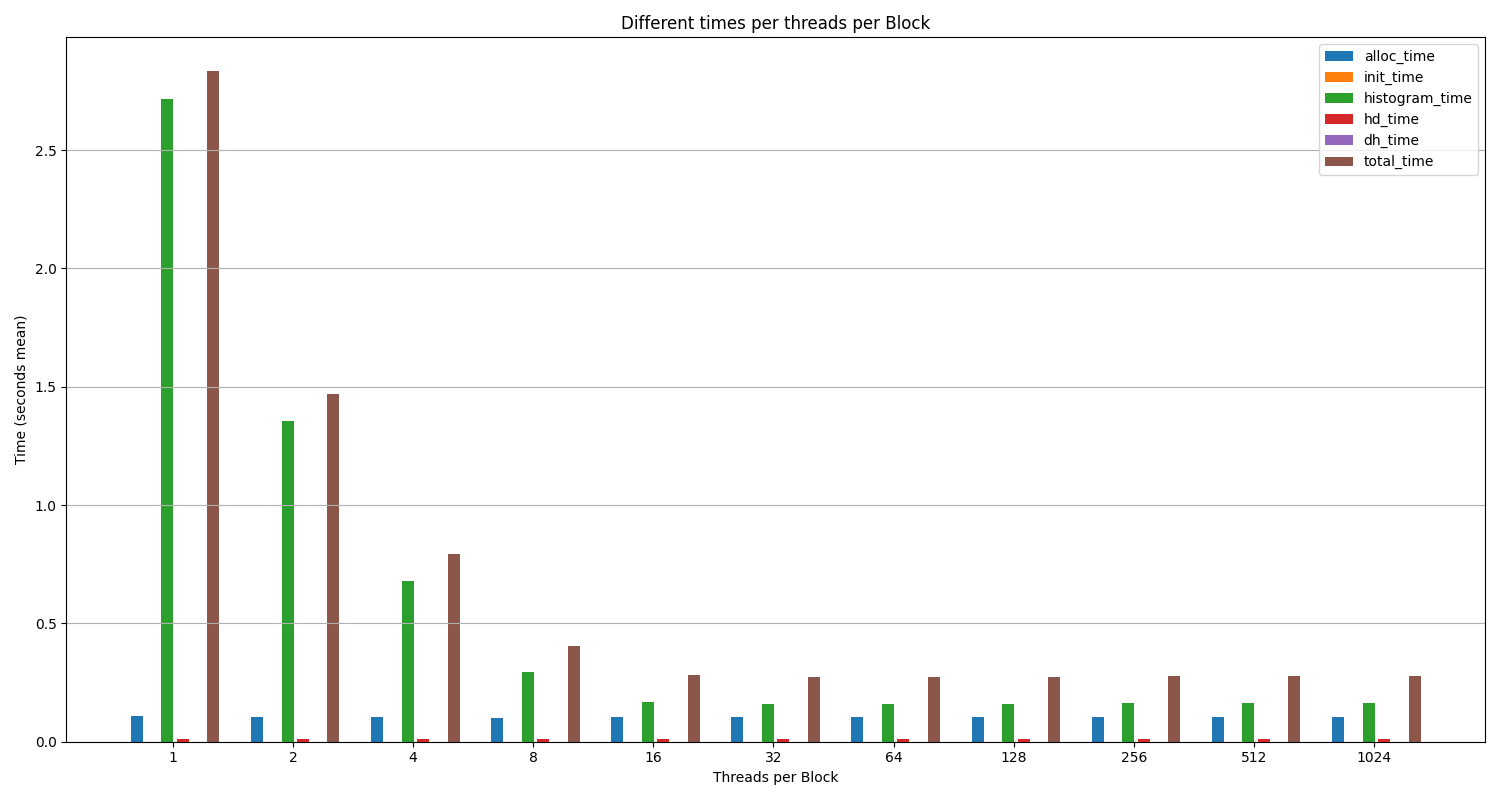
\includegraphics[width=0.9\textwidth]{images/histogram_1/times_per_threadsPerBlock.png}
            }
            \caption{Tiempos de ejecución según el tamaño de bloque usando memoria global.}
            \label{fig:histogram_times_per_threadsPerBlock_global}
        \end{figure}
        
        \begin{figure}[H]
            \centering
            \fbox{
                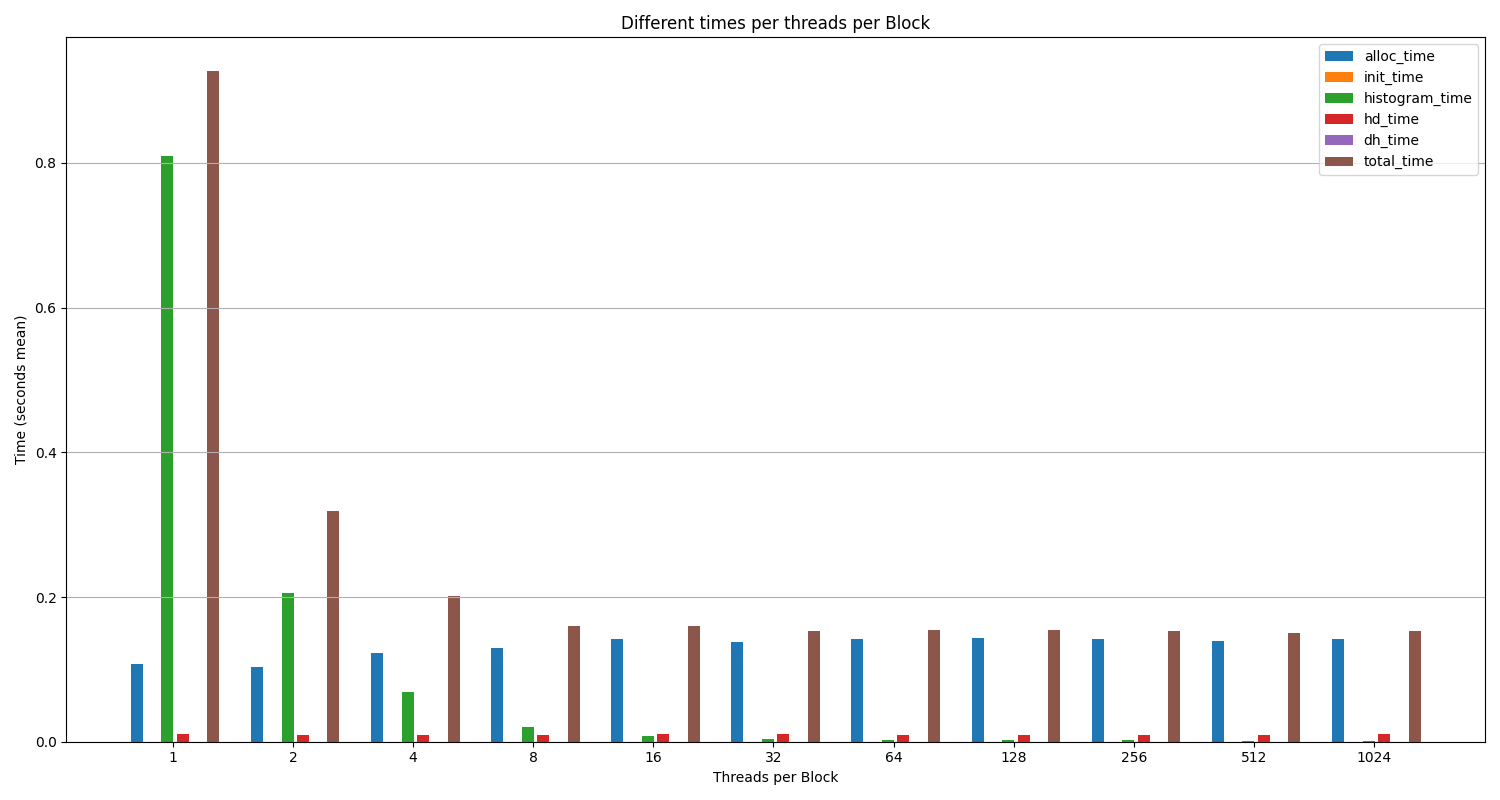
\includegraphics[width=0.9\textwidth]{images/histogram_2/times_per_threadsPerBlock.png}
            }
            \caption{Tiempos de ejecución según el tamaño de bloque usando memoria compartida.}
            \label{fig:histogram_times_per_threadsPerBlock_shared}
        \end{figure}
        
        En la implementación con memoria global (figura \ref{fig:histogram_times_per_threadsPerBlock_global}), se observa un comportamiento característico donde el tiempo de ejecución disminuye drásticamente al aumentar el número de \textit{threads} por bloque. Con un solo \textit{thread} por bloque, el tiempo total supera los 2.8 segundos, dominado principalmente por el tiempo de cálculo del histograma (\texttt{histogram\_time}) que alcanza aproximadamente 2.7 segundos. Al incrementar a 2 \textit{threads} por bloque, el tiempo total se reduce a aproximadamente 1.5 segundos, con el tiempo de cálculo del histograma reduciéndose a 1.35 segundos. Esta tendencia decreciente continúa hasta llegar a los 16 \textit{threads} por bloque, donde el tiempo total se estabiliza alrededor de 0.3 segundos.
        
        A partir de 32 \textit{threads} por bloque, se observa que el tiempo total se mantiene prácticamente constante en torno a 0.25-0.30 segundos, lo que sugiere que se ha alcanzado el límite de paralelismo efectivo para esta implementación y este conjunto de datos específico. Es destacable que el tiempo de cálculo del histograma (\texttt{histogram\_time}) sigue siendo el componente dominante del tiempo total, aunque su proporción disminuye a medida que aumenta el número de \textit{threads} por bloque.
        
        En contraste, la implementación con memoria compartida (figura \ref{fig:histogram_times_per_threadsPerBlock_shared}) muestra un comportamiento significativamente diferente. El tiempo total máximo con un solo \textit{thread} por bloque es de aproximadamente 0.95 segundos, considerablemente menor que en la implementación con memoria global. El tiempo de cálculo del histograma en este caso es de alrededor de 0.8 segundos, también notablemente inferior.
        La reducción en el tiempo total al aumentar el número de \textit{threads} por bloque es más pronunciada en esta implementación. Con 8 \textit{threads} por bloque, el tiempo total ya se ha reducido a aproximadamente 0.16 segundos, y a partir de 16 \textit{threads} por bloque, se estabiliza en torno a 0.15 segundos. Un aspecto particularmente interesante es que a partir de 16 \textit{threads} por bloque, el tiempo de cálculo del histograma (\texttt{histogram\_time}) se vuelve prácticamente insignificante (apenas visible en la gráfica), mientras que el tiempo de asignación de memoria (\texttt{alloc\_time}) pasa a ser el componente dominante del tiempo total.
        
        Comparando ambas implementaciones, se pueden extraer varias conclusiones importantes:

        \begin{enumerate}

            \item \textbf{Eficiencia general}: La implementación con memoria compartida es significativamente más eficiente que la implementación con memoria global, con tiempos totales aproximadamente 2-3 veces menores para configuraciones equivalentes.
            
            \item \textbf{Escalabilidad}: Ambas implementaciones muestran una mejora significativa al aumentar el número de \textit{threads} por bloque hasta un cierto punto (16-32 \textit{threads}), después del cual la mejora es marginal o inexistente. Esto sugiere que se alcanza un límite de paralelismo efectivo relacionado con la arquitectura de la GPU utilizada.
            
            \item \textbf{Cuello de botella}: En la implementación con memoria global, el tiempo de cálculo del histograma sigue siendo considerable incluso con un alto número de \textit{threads} por bloque. En cambio, en la implementación con memoria compartida, este tiempo se vuelve insignificante, y el cuello de botella pasa a ser la asignación de memoria y las transferencias entre \textit{host} y \textit{device}.
            
            \item \textbf{Efecto de la memoria compartida}: La drástica reducción del tiempo de cálculo del histograma en la implementación con memoria compartida demuestra la eficacia de esta técnica para reducir la latencia de acceso a memoria y minimizar los conflictos en las operaciones atómicas.
            
            \item \textbf{\textit{Overhead} de inicialización}: En ambas implementaciones, con un alto número de \textit{threads} por bloque, los tiempos de transferencia de datos (\texttt{hd\_time} y\texttt{dh\_time}) y de inicialización (\texttt{init\_time}) pasan a ser componentes significativos del tiempo total, lo que sugiere que, para problemas de mayor tamaño, estrategias como el solapamiento de cómputo y comunicación podrían ser beneficiosas.
                     
        \end{enumerate}
        
        En resumen, estos resultados confirman la importancia de la optimización de acceso a memoria en aplicaciones CUDA, especialmente en algoritmos como el cálculo de histogramas que involucran operaciones atómicas y patrones de acceso a memoria potencialmente conflictivos. La implementación con memoria compartida demuestra ser claramente superior, reduciendo significativamente el tiempo de ejecución y mejorando la escalabilidad con respecto al número de \textit{threads} por bloque.
       
    \subsection{Ocupancia}

        La figura \ref{fig:histogram_ioccupancy_per_threadsPerBlock} muestra cómo la ocupancia teórica de los multiprocesadores de la GPU (SM) varía en función del número de hilos por bloque, proporcionando información clave sobre la utilización de los recursos disponibles.

        \begin{figure}[H]
            \centering
            \fbox{
                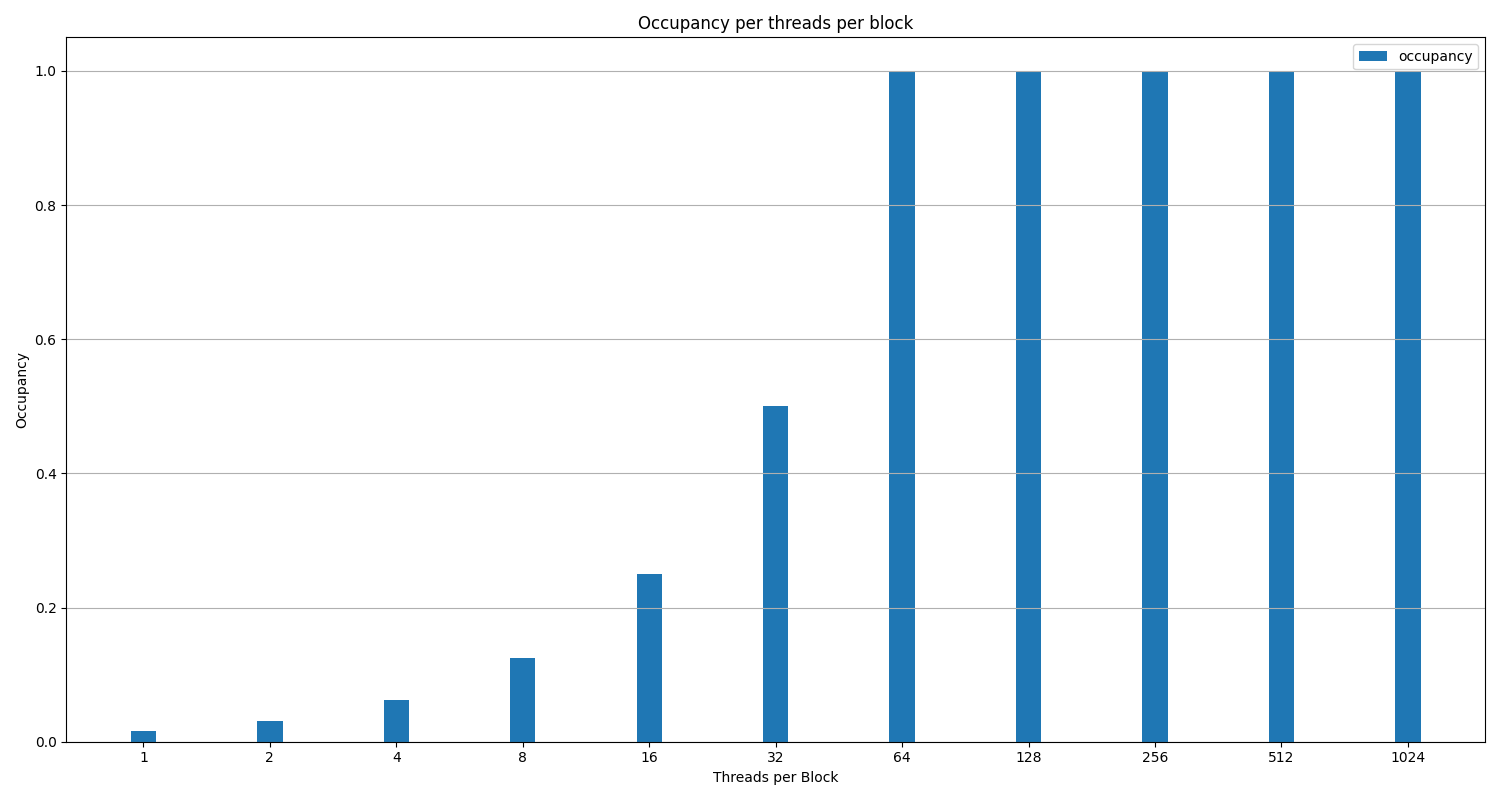
\includegraphics[width=0.9\textwidth]{images/histogram_1/occupancy_per_threadsPerBlock.png}
            }
            \caption{Ocupancia según el tamaño de bloque.}
            \label{fig:histogram_ioccupancy_per_threadsPerBlock}
        \end{figure}

        \begin{itemize}
        
            \item En configuraciones con un número reducido de hilos por bloque (1-32), la ocupancia es muy baja (inferior a 0.5), lo que explica el bajo rendimiento observado en estos casos. Una ocupancia reducida impide que el \textit{hardware} oculte de manera eficiente las latencias de acceso a memoria mediante el cambio de contexto entre \textit{warps}, resultando en una ejecución poco eficiente.
            
            \item Se observa un punto de inflexión importante en la configuración de 64 hilos por bloque, donde la ocupancia alcanza el valor máximo de 1.0 (100\%). Este valor se mantiene constante para configuraciones de mayor tamaño (128, 256, 512 y 1024 hilos por bloque). Este comportamiento está relacionado con los algoritmos de cálculo de ocupancia implementados en el código. Una ocupancia máxima indica que la GPU mantiene suficientes bloques activos por SM para aprovechar completamente los recursos de ejecución, lo que en teoría debería conducir a un rendimiento óptimo.
            
            \item A pesar de alcanzar una ocupancia perfecta a partir de 64 hilos por bloque, el mejor rendimiento (según la figura 1) se obtiene con configuraciones de 128-256 hilos por bloque. Esta diferencia sugiere que la ocupancia teórica no es el único factor determinante del rendimiento práctico. Factores como el tamaño del conjunto de trabajo en cachés L1/L2, la eficiencia en la coalescencia de accesos a memoria y la divergencia de \textit{warps} también influyen significativamente en el rendimiento global.
            
        \end{itemize}
        
    \subsection{Matriz de isoeficiencia}

        Las figuras \ref{fig:histogram_isoeficiency_global} y \ref{fig:histogram_isoeficiency_shared} muestran matrices de isoeficiencia que ofrecen una perspectiva integral y multidimensional del rendimiento, considerando dos variables clave: el tamaño del problema en el eje horizontal, representado por las distintas imágenes examinadas y la cantidad de hilos por bloque en el eje vertical. Esta representación avanzada facilita la identificación de áreas con eficiencia similar en distintas configuraciones.

        \begin{figure}[H]
            \centering
            \fbox{
                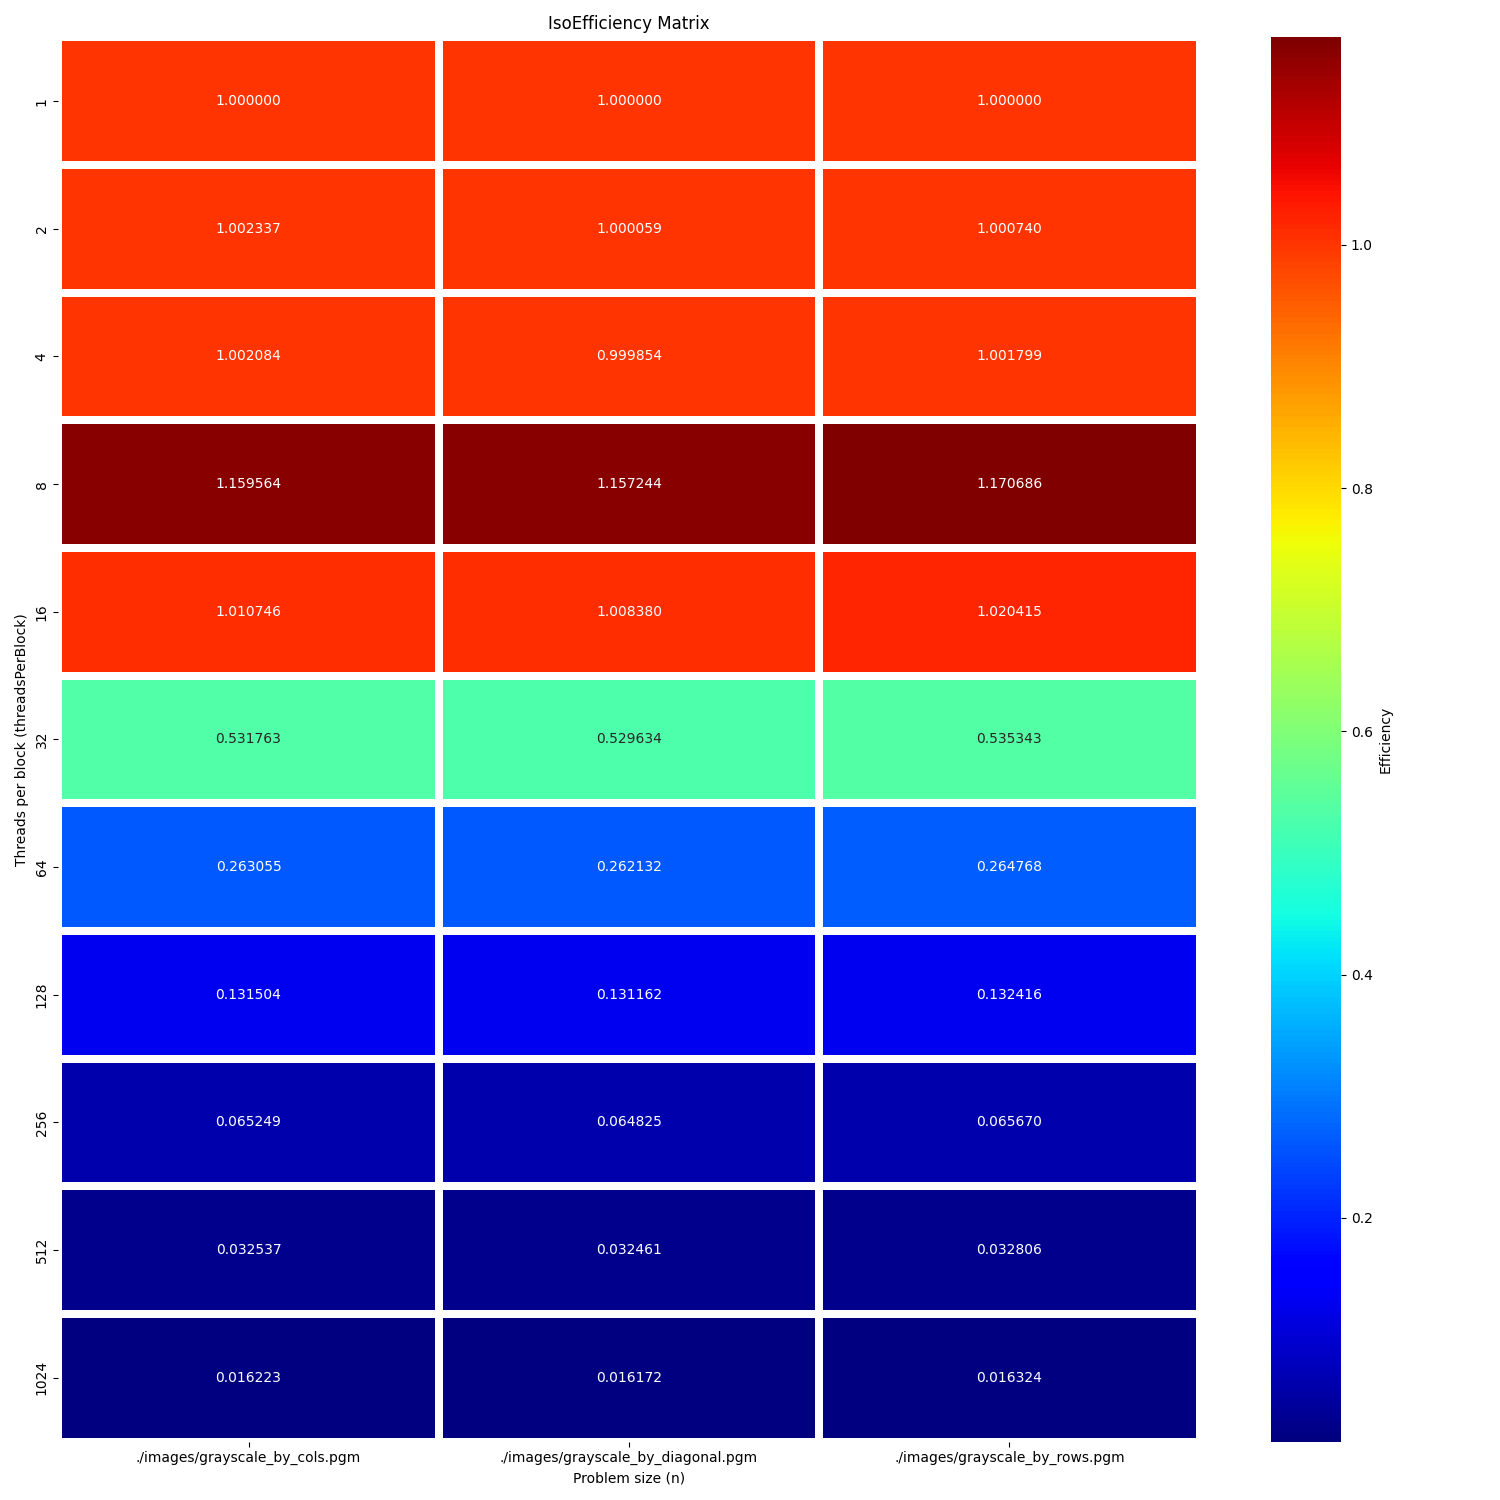
\includegraphics[width=0.9\textwidth]{images/histogram_1/isoEfficiencyMatrix.png}
            }
            \caption{Matriz de isoeficiencia usando memoria global.}
            \label{fig:histogram_isoeficiency_global}
        \end{figure}  

        \begin{figure}[H]
            \centering
            \fbox{
                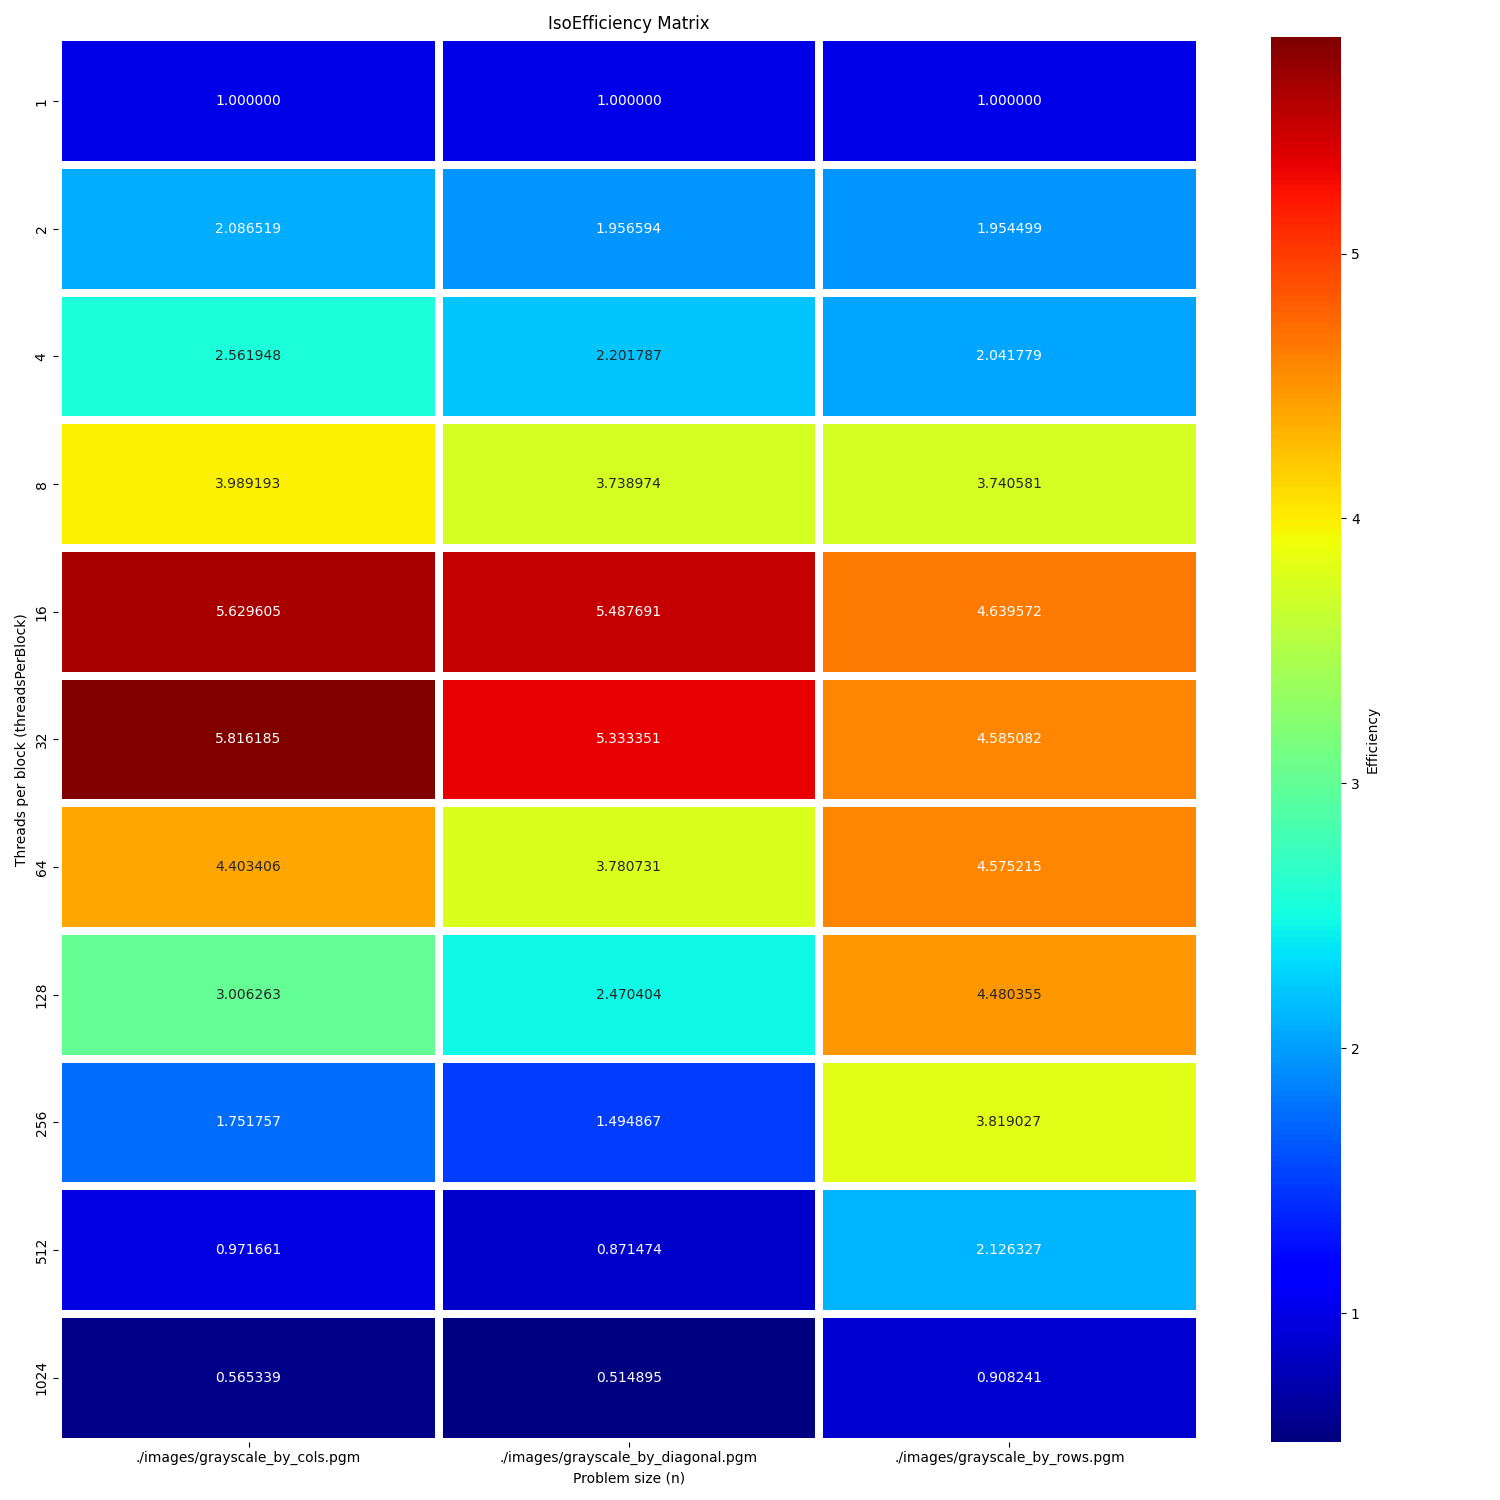
\includegraphics[width=0.9\textwidth]{images/histogram_2/isoEfficiencyMatrix.png}
            }
            \caption{Matriz de isoeficiencia usando memoria compartida.}
            \label{fig:histogram_isoeficiency_shared}
        \end{figure}

        En la matriz de isoeficiencia para la implementación con memoria global (figura \ref{fig:histogram_isoeficiency_global}), se observa una tendencia donde la eficiencia aumenta significativamente con tamaños de problema mayores y configuraciones de hilos intermedias. Los valores más altos de eficiencia (representados por colores rojo oscuro) se concentran en configuraciones con 16 y 32 hilos por bloque, alcanzando valores superiores a 5.0. Esto sugiere que estas configuraciones logran un mejor aprovechamiento de los recursos de la GPU para problemas de tamaño medio y grande.
        
        Por otro lado, la matriz de isoeficiencia para la implementación con memoria compartida (figura \ref{fig:histogram_isoeficiency_shared}) muestra un patrón claramente diferente. La eficiencia máxima se concentra en las configuraciones con pocos hilos (1-8) y disminuye drásticamente conforme aumenta el número de hilos por bloque. Los valores más altos apenas superan 1.0, lo que indica que la implementación con memoria compartida no escala tan bien como la global en términos de eficiencia paralela.
        
        Es notable que la eficiencia en la implementación con memoria compartida decrece exponencialmente con el aumento del número de hilos, llegando a valores por debajo de 0.1 para configuraciones con 256 hilos o más. Esto podría atribuirse a conflictos de acceso a memoria compartida o a una saturación de recursos cuando se utilizan demasiados hilos simultáneamente.

        Comparando ambas matrices, se puede concluir que la implementación con memoria global ofrece mejor escalabilidad y eficiencia para un rango más amplio de configuraciones, especialmente para problemas de mayor tamaño. La implementación con memoria compartida, aunque potencialmente más rápida en términos absolutos, muestra limitaciones significativas en su capacidad de escalar eficientemente con el aumento de recursos paralelos.
        
    \subsection{Métricas generales}

        \begin{table}[H]
            \centering
            \begin{adjustbox}{width=\textwidth, keepaspectratio}
                \begin{tabular}{rlrrrrrrr}
                    \toprule
                    Threads & Image Path & Max Time & Ref Time & Speedup & Efficiency & Quality & Secuential Compute Speedup & Secuential Total Speedup \\
                    \midrule
                    1 & ./images/grayscale\_by\_cols.pgm & 2.72 & 2.72 & 1.00 & 1.00 & 0.37 & 0.08 & 0.22 \\
                    2 & ./images/grayscale\_by\_cols.pgm & 1.36 & 2.72 & 2.00 & 1.00 & 0.74 & 0.15 & 0.43 \\
                    4 & ./images/grayscale\_by\_cols.pgm & 0.68 & 2.72 & 4.01 & 1.00 & 1.47 & 0.30 & 0.80 \\
                    8 & ./images/grayscale\_by\_cols.pgm & 0.29 & 2.72 & 9.28 & 1.16 & 3.41 & 0.70 & 1.56 \\
                    16 & ./images/grayscale\_by\_cols.pgm & 0.17 & 2.72 & 16.17 & 1.01 & 5.94 & 1.22 & 2.22 \\
                    32 & ./images/grayscale\_by\_cols.pgm & 0.16 & 2.72 & 17.02 & 0.53 & 6.25 & 1.28 & 2.30 \\
                    64 & ./images/grayscale\_by\_cols.pgm & 0.16 & 2.72 & 16.84 & 0.26 & 6.19 & 1.27 & 2.27 \\
                    128 & ./images/grayscale\_by\_cols.pgm & 0.16 & 2.72 & 16.83 & 0.13 & 6.19 & 1.27 & 2.28 \\
                    256 & ./images/grayscale\_by\_cols.pgm & 0.16 & 2.72 & 16.70 & 0.07 & 6.14 & 1.26 & 2.25 \\
                    512 & ./images/grayscale\_by\_cols.pgm & 0.16 & 2.72 & 16.66 & 0.03 & 6.12 & 1.25 & 2.09 \\
                    1024 & ./images/grayscale\_by\_cols.pgm & 0.16 & 2.72 & 16.61 & 0.02 & 6.11 & 1.25 & 2.24 \\
                    1 & ./images/grayscale\_by\_diagonal.pgm & 2.71 & 2.71 & 1.00 & 1.00 & 0.37 & 0.08 & 0.22 \\
                    2 & ./images/grayscale\_by\_diagonal.pgm & 1.36 & 2.71 & 2.00 & 1.00 & 0.74 & 0.15 & 0.43 \\
                    4 & ./images/grayscale\_by\_diagonal.pgm & 0.68 & 2.71 & 4.00 & 1.00 & 1.47 & 0.30 & 0.80 \\
                    8 & ./images/grayscale\_by\_diagonal.pgm & 0.29 & 2.71 & 9.26 & 1.16 & 3.41 & 0.70 & 1.48 \\
                    16 & ./images/grayscale\_by\_diagonal.pgm & 0.17 & 2.71 & 16.13 & 1.01 & 5.94 & 1.22 & 2.22 \\
                    32 & ./images/grayscale\_by\_diagonal.pgm & 0.16 & 2.71 & 16.95 & 0.53 & 6.24 & 1.28 & 2.27 \\
                    64 & ./images/grayscale\_by\_diagonal.pgm & 0.16 & 2.71 & 16.78 & 0.26 & 6.18 & 1.26 & 2.28 \\
                    128 & ./images/grayscale\_by\_diagonal.pgm & 0.16 & 2.71 & 16.79 & 0.13 & 6.18 & 1.26 & 2.30 \\
                    256 & ./images/grayscale\_by\_diagonal.pgm & 0.16 & 2.71 & 16.60 & 0.06 & 6.11 & 1.25 & 2.26 \\
                    512 & ./images/grayscale\_by\_diagonal.pgm & 0.16 & 2.71 & 16.62 & 0.03 & 6.12 & 1.25 & 2.25 \\
                    1024 & ./images/grayscale\_by\_diagonal.pgm & 0.16 & 2.71 & 16.56 & 0.02 & 6.10 & 1.25 & 2.24 \\
                    1 & ./images/grayscale\_by\_rows.pgm & 2.73 & 2.73 & 1.00 & 1.00 & 0.37 & 0.08 & 0.22 \\
                    2 & ./images/grayscale\_by\_rows.pgm & 1.36 & 2.73 & 2.00 & 1.00 & 0.73 & 0.15 & 0.43 \\
                    4 & ./images/grayscale\_by\_rows.pgm & 0.68 & 2.73 & 4.01 & 1.00 & 1.47 & 0.30 & 0.80 \\
                    8 & ./images/grayscale\_by\_rows.pgm & 0.29 & 2.73 & 9.37 & 1.17 & 3.44 & 0.70 & 1.56 \\
                    16 & ./images/grayscale\_by\_rows.pgm & 0.17 & 2.73 & 16.33 & 1.02 & 5.99 & 1.22 & 2.20 \\
                    32 & ./images/grayscale\_by\_rows.pgm & 0.16 & 2.73 & 17.13 & 0.54 & 6.29 & 1.29 & 2.08 \\
                    64 & ./images/grayscale\_by\_rows.pgm & 0.16 & 2.73 & 16.95 & 0.26 & 6.22 & 1.27 & 2.27 \\
                    128 & ./images/grayscale\_by\_rows.pgm & 0.16 & 2.73 & 16.95 & 0.13 & 6.22 & 1.27 & 2.26 \\
                    256 & ./images/grayscale\_by\_rows.pgm & 0.16 & 2.73 & 16.81 & 0.07 & 6.17 & 1.26 & 2.26 \\
                    512 & ./images/grayscale\_by\_rows.pgm & 0.16 & 2.73 & 16.80 & 0.03 & 6.16 & 1.26 & 2.27 \\
                    1024 & ./images/grayscale\_by\_rows.pgm & 0.16 & 2.73 & 16.72 & 0.02 & 6.13 & 1.25 & 2.26 \\
                    \bottomrule
                \end{tabular}
            \end{adjustbox}
            \caption{Métricas generales usando memoria global.}
            \label{tab:histogram_metrics_global}
        \end{table}

        \begin{table}[H]
            \centering
            \begin{adjustbox}{width=\textwidth, keepaspectratio}
                \begin{tabular}{rlrrrrrrr}
                    \toprule
                    Threads & Image Path & Max Time & Ref Time & Speedup & Efficiency & Quality & Secuential Compute Speedup & Secuential Total Speedup \\
                    \midrule
                    1 & ./images/grayscale\_by\_cols.pgm & 0.86 & 0.86 & 1.00 & 1.00 & 1.16 & 0.24 & 0.62 \\
                    2 & ./images/grayscale\_by\_cols.pgm & 0.21 & 0.86 & 4.17 & 2.09 & 4.86 & 0.99 & 1.93 \\
                    4 & ./images/grayscale\_by\_cols.pgm & 0.08 & 0.86 & 10.25 & 2.56 & 11.93 & 2.44 & 2.70 \\
                    8 & ./images/grayscale\_by\_cols.pgm & 0.03 & 0.86 & 31.91 & 3.99 & 37.16 & 7.60 & 3.19 \\
                    16 & ./images/grayscale\_by\_cols.pgm & 0.01 & 0.86 & 90.07 & 5.63 & 104.88 & 21.45 & 3.63 \\
                    32 & ./images/grayscale\_by\_cols.pgm & 0.00 & 0.86 & 186.12 & 5.82 & 216.70 & 44.32 & 3.75 \\
                    64 & ./images/grayscale\_by\_cols.pgm & 0.00 & 0.86 & 281.82 & 4.40 & 328.13 & 67.10 & 2.85 \\
                    128 & ./images/grayscale\_by\_cols.pgm & 0.00 & 0.86 & 384.80 & 3.01 & 448.04 & 91.62 & 3.76 \\
                    256 & ./images/grayscale\_by\_cols.pgm & 0.00 & 0.86 & 448.45 & 1.75 & 522.15 & 106.78 & 3.67 \\
                    512 & ./images/grayscale\_by\_cols.pgm & 0.00 & 0.86 & 497.49 & 0.97 & 579.25 & 118.46 & 3.92 \\
                    1024 & ./images/grayscale\_by\_cols.pgm & 0.00 & 0.86 & 578.91 & 0.57 & 674.04 & 137.84 & 3.96 \\
                    1 & ./images/grayscale\_by\_diagonal.pgm & 0.81 & 0.81 & 1.00 & 1.00 & 1.24 & 0.25 & 0.69 \\
                    2 & ./images/grayscale\_by\_diagonal.pgm & 0.21 & 0.81 & 3.91 & 1.96 & 4.86 & 0.99 & 1.97 \\
                    4 & ./images/grayscale\_by\_diagonal.pgm & 0.09 & 0.81 & 8.81 & 2.20 & 10.93 & 2.24 & 2.67 \\
                    8 & ./images/grayscale\_by\_diagonal.pgm & 0.03 & 0.81 & 29.91 & 3.74 & 37.14 & 7.59 & 3.28 \\
                    16 & ./images/grayscale\_by\_diagonal.pgm & 0.01 & 0.81 & 87.80 & 5.49 & 109.01 & 22.29 & 3.60 \\
                    32 & ./images/grayscale\_by\_diagonal.pgm & 0.00 & 0.81 & 170.67 & 5.33 & 211.89 & 43.33 & 3.76 \\
                    64 & ./images/grayscale\_by\_diagonal.pgm & 0.00 & 0.81 & 241.97 & 3.78 & 300.42 & 61.44 & 3.72 \\
                    128 & ./images/grayscale\_by\_diagonal.pgm & 0.00 & 0.81 & 316.21 & 2.47 & 392.60 & 80.29 & 3.84 \\
                    256 & ./images/grayscale\_by\_diagonal.pgm & 0.00 & 0.81 & 382.69 & 1.49 & 475.13 & 97.16 & 3.73 \\
                    512 & ./images/grayscale\_by\_diagonal.pgm & 0.00 & 0.81 & 446.19 & 0.87 & 553.98 & 113.29 & 3.88 \\
                    1024 & ./images/grayscale\_by\_diagonal.pgm & 0.00 & 0.81 & 527.25 & 0.51 & 654.61 & 133.87 & 3.77 \\
                    1 & ./images/grayscale\_by\_rows.pgm & 0.80 & 0.80 & 1.00 & 1.00 & 1.24 & 0.25 & 0.69 \\
                    2 & ./images/grayscale\_by\_rows.pgm & 0.21 & 0.80 & 3.91 & 1.95 & 4.86 & 0.99 & 1.96 \\
                    4 & ./images/grayscale\_by\_rows.pgm & 0.10 & 0.80 & 8.17 & 2.04 & 10.15 & 2.08 & 2.45 \\
                    8 & ./images/grayscale\_by\_rows.pgm & 0.03 & 0.80 & 29.92 & 3.74 & 37.20 & 7.61 & 3.34 \\
                    16 & ./images/grayscale\_by\_rows.pgm & 0.01 & 0.80 & 74.23 & 4.64 & 92.27 & 18.87 & 3.72 \\
                    32 & ./images/grayscale\_by\_rows.pgm & 0.01 & 0.80 & 146.72 & 4.59 & 182.37 & 37.30 & 3.87 \\
                    64 & ./images/grayscale\_by\_rows.pgm & 0.00 & 0.80 & 292.81 & 4.58 & 363.97 & 74.43 & 3.89 \\
                    128 & ./images/grayscale\_by\_rows.pgm & 0.00 & 0.80 & 573.49 & 4.48 & 712.84 & 145.78 & 3.78 \\
                    256 & ./images/grayscale\_by\_rows.pgm & 0.00 & 0.80 & 977.67 & 3.82 & 1215.24 & 248.52 & 3.93 \\
                    512 & ./images/grayscale\_by\_rows.pgm & 0.00 & 0.80 & 1088.68 & 2.13 & 1353.22 & 276.73 & 3.98 \\
                    1024 & ./images/grayscale\_by\_rows.pgm & 0.00 & 0.80 & 930.04 & 0.91 & 1156.03 & 236.41 & 3.96 \\
                    \bottomrule
                \end{tabular}
            \end{adjustbox}
            \caption{Métricas generales usando memoria compartida.}
            \label{tab:histogram_metrics_shared}
        \end{table} 
